\section{Standardisierung der Schnittstellennavigation}

Dieser Teil konzentriert sich auf die Umsetzung der im Abschnitt \ref{sec:analyse-navigation} definierten Lösungen und verwendet hauptsächlich die im Abschnitt \ref{sec:angular} erwähnten Funktionen des Angular-Frameworks.

\subsection{Seitentitel als Service}

Der Seitentitel sollte an zwei verschiedenen Stellen auf der Seite verwendet werden: im Header der Seite, wo sich das Icon der Benutzeroberfläche befindet, und im Tabulatortitel der Anwendung, wo sich das Favicon befindet.
Angular bietet bereits einen Service \lstinline{Title}, mit dem der Titel der Anwendung geändert werden kann.
Es ist daher sinnvoll, einen neuen Service \lstinline{PageTitleService} zu definieren, der den Basisservice \lstinline{Title} verwendet, und den Titel in einer dynamischen Variablen zu speichern, die in der Schablone der Komponente \lstinline{header} verwendet werden kann.

Dieser Service sollte auch den \lstinline{Router} Service verwenden, der es ermöglicht, mithilfe eines \lstinline{Observers} auf Änderungen der URL der Anwendung zu hören.
\begin{lstlisting}[
  language=javascript,
  caption={Vereinfachte Struktur des Service \lstinline{PageTitle}},
  captionpos=b,
  label={lst:page_title_service}
]
@Injectable({
  providedIn: "root",
})
export class PageTitleService {
  private DEFAULT_TITLE = "Dryad"
  private TITLE_APPEND = " * Dryad"

  public pageTitle: string

  constructor(
    private titleService: Title,
    private router: Router
  ) {
    this.initRouterObserver()
  }

  private initRouterObserver(): void {
    this.router.events
      .pipe(filter((event: Event) => event instanceof NavigationEnd))
      .subscribe((event: NavigationEnd) => {
        // update page title when url is changed
        this.setTitleForSlug(event.url)
      })
  }

  private setTitleForSlug(slug: string): void {
    // ...
  }

  public setDefault(): void {
    this.titleService.setTitle(this.DEFAULT_TITLE)
  }

  public set(title: string): void {
    this.titleService.setTitle(title + this.TITLE_APPEND)
  }
}
\end{lstlisting}

Der Router der Anwendung basiert auf \ac{URI}s, die in einer statischen Klasse \lstinline{DryadRoutes} vordefiniert sind.
Die Strategie der \lstinline{setTitleForSlug}-Methode besteht darin, zu überprüfen, ob der angegebene \ac{URI} mit einem der vordefinierten \ac{URI}s beginnt.
Dies muss leider unter \lstinline{if-else}-Bedingungen geschehen, da die \ac{URI}s nach dem \ac{REST}-Standard verlängert werden.
Daher ist es notwendig, dass ein Test auf einer tieferen Route wie \lstinline{/users/:userId/settings} vor einer anderen wie \lstinline{/users} durchgeführt wird.

\begin{lstlisting}[
  language=javascript,
  caption={Vereinfachter Code für die Methode \lstinline{setTitleForSlug} der Klasse \lstinline{PageTitleService} (siehe \ref{lst:page_title_service}) },
  captionpos=b,
  label={lst:setTitleForSlug}
]
private setTitleForSlug(slug: string): void {
  this.pageTitle = undefined
  let appTitle

  if (slug.startsWith(DryadRoutes.DASHBOARD)) {
    appTitle = "Dashboard"
    this.pageTitle = "Dashboard"
  } else if (slug.startsWith(DryadRoutes.SITES)) {
    appTitle = "Sites"
    this.pageTitle = "Site Management"
  } else {
    // ...
  }

  if (appTitle) this.set(appTitle)
  else this.setDefault()
}
\end{lstlisting}

Auf diese Weise kann die \lstinline{Header}-Komponente den Service in ihren Konstruktor importieren, um die dynamische Variable \lstinline{pageTitle} direkt in ihrem Template zu verwenden:

\begin{lstlisting}[
  language=html,
  caption={Verwendung des \lstinline{PageTitleService} in der \lstinline{Header}-Komponente},
  captionpos=b
]
<h1 class="app-name">{{ pageTitleService.pageTitle }}</h1>
\end{lstlisting}


\subsection{Individuelle und dauerhafte Anzeige der Schnittstelle}

Wie im Abschnitt \ref{sec:navigationssystem} erwähnt, sollte die Sidebar in der Lage sein, die Beschriftung der Menüpunkte anzuzeigen oder nicht.

\subsubsection{Menü-Rendering}

Das Menü wird aus einer Liste von Elementen des Typs \lstinline{MenuItem} im Komponent \lstinline{SideBarMenuComponent} generiert:

\begin{lstlisting}[
  language=javascript,
  caption={Definition der TypeScript-Interface \lstinline{MenuItem}},
  captionpos=b,
  label={lst:menuitem_interface}
]
interface MenuItem {
  icon: string
  slug: DryadRoutes
  label: string
}
\end{lstlisting}

Das Hinzufügen einer dynamischen Variablen \lstinline{showLabels} im Controller mit der Verwendung der Syntax \lstinline{*ngIf="showLabels"} in der Template ermöglicht es, die Labels einfach anzuzeigen oder nicht anzuzeigen.
Am Ende der Liste wird eine Schaltfläche \lstinline{<button>} platziert, mit der Sie den booleschen Wert von \lstinline{showLabels} umschalten können.

\begin{lstlisting}[
  language=html,
  caption={Vereinfachte Ansicht des Menü-Templates},
  captionpos=b
]
<div>
  <ul>
    <li *ngFor="let menuItem of MENU_ITEMS">
      <a
        [routerLink]="menuItem.slug"
        title="{{ menuItem.label }}"
      >
        <i class="{{ menuItem.icon }}"></i>
        <span class="label" *ngIf="showLabels">{{ menuItem.label }}</span>
      </a>
    </li>
  </ul>

  <button (click)="toggleShowLabels()">
    <i class="ph-caret-double-left" [ngClass]="{ 'rotate-180': !showLabels }"></i>
    <span class="label">Collapse</span>
  </button>
</div>
\end{lstlisting}

\subsubsection{Konsistente Schnittstelle}

Die Variable \lstinline{showLabels} ist im Controller standardmäßig auf \lstinline{true} gesetzt.
Da dieser Controller in JavaScript-Code geschrieben ist, der auf dem Gerät des Benutzers ausgeführt wird, ist es nicht möglich, den zuletzt verwendeten Wert zwischen verschiedenen Sitzungen zu speichern.
Wenn die Seite also aktualisiert wird, wird der Wert von \lstinline{showLabels} wieder auf \lstinline{true} gesetzt.
Daher ist es notwendig, eine sitzungsübergreifende Logik zur Speicherung von Informationen zu implementieren.

Eine der am meisten beantworteten ist die Speicherung der Settings des Benutzers mithilfe eines Backend Service, der eine Datenbank verwaltet, die er lesen und verändern kann.
Dies hat den großen Vorteil, dass es zentralisiert ist, so dass die Einstellungen für alle unterschiedlichen Geräte des Nutzers gleich sind.
Leider ist Dryad nicht in der Lage, einen solchen Service in der zur Verfügung stehenden Zeit zu entwickeln.

Glücklicherweise ermöglicht der Browser mittels \lstinline{localstorage} die lokale Speicherung von Daten für eine bestimmte Website\cite{localstorage}.
Die Nur-Lese-Eigenschaft localStorage der Fensterschnittstelle ermöglicht den Zugriff auf ein Speicherobjekt für den Ursprung des Dokuments; die gespeicherten Daten werden über Browser-Sitzungen hinweg gespeichert.
Es ist also möglich, den Wert von showLabels einfach im localStorage zu speichern und ihn wieder einzulesen, wenn die Komponente initialisiert wird.
Um das Rad nicht neu erfinden zu müssen, wird dies über einen einfachen TypeScript-Decorator \lstinline{@LocalStorage} ermöglicht, der vom Open-Source-Projekt \lstinline{ngx-store}\footnote{Siehe \href{https://github.com/zoomsphere/ngx-store}{https://github.com/zoomsphere/ngx-store}} entwickelt wurde.

Der folgende Code erstellt im Controller eine dynamische Variable \lstinline{showLabels}, die den Standardwert true hat, wenn kein Element im \lstinline{localstorage} durch den Namen \lstinline{sidebar-with-labels} identifiziert wird.
Wenn es einen Eintrag gibt, wird die Variable auf den booleschen Wert dieses Eintrags gesetzt.

\begin{lstlisting}[
  language=javascript,
  caption={Code für die Deklaration der Variablen \lstinline{showLabels}},
  captionpos=b
]
@LocalStorage('sidebar-with-labels') showLabels = true
\end{lstlisting}

\subsection{REST-Routing mit Angular}

Wie im Abschnitt \ref{sec:hierarchie_anwendung} erwähnt, muss die Anwendung die verschiedenen Seiten nach dem \ac{REST}-Standard darstellen.
Daher ist es notwendig, die verschiedenen Komponenten als Seite zu klassifizieren, die über einen einzigen \ac{URI} erreichbar ist.

Diese Implementierung ist über den Router von Angular recht einfach zu implementieren.
Anstatt einfach nur eine komplette Schnittstelle mit einer URL zu verknüpfen, kann man festlegen, dass sich nur ein Teilstück einer sogenannten Layout-Komponente ändert.
So können Sie z. B. den \lstinline{Header} und die \lstinline{Sidebar} immer anzeigen, ohne sie in jede Komponente der Seite einfügen zu müssen.

\begin{lstlisting}[
  language=javascript,
  caption={Konfiguration des Routers mit einem Hauptlayout \lstinline{MainLayoutComponent}},
  captionpos=b
]
{
  path: "",
  component: MainLayoutComponent,
  children: [
    { path: DryadRoutes.DASHBOARD, component: DashboardComponent },
    { path: DryadRoutes.SITES, component: SiteListComponent },
    // ...
  ],
}
\end{lstlisting}

Dieses Schema mit dem Objekt \lstinline{children} kann rekursiv wiederholt werden, so dass die Route \lstinline{/sites/:siteId/sensors} die Komponente \lstinline{SiteSensorsListComponent} auf diese Weise anzeigen kann:

\begin{lstlisting}[
  language=javascript,
  caption={Beispiel für ein verschachteltes Routing-Schema mit dem Router von Angular},
  captionpos=b
]
{
  path: "",
  component: MainLayoutComponent,
  children: [
    { 
      path: DryadRoutes.SITES, // /sites
      component: SiteListComponent,
      children: [
        { 
          path: DryadRoutes.SITE, // /:siteId
          component: SiteComponent,
          children: [
            { 
              path: DryadRoutes.SENSORS, // /sensors
              component: SiteSensorsListComponent
            },
            // ...
          ],
        },
        // ...
      ],
    },
    // ...
  ],
}
\end{lstlisting}

Diese Funktion des Routers hat es ermöglicht, leicht von einer Architektur wie \ref{fig:site_map} zu \ref{fig:site_map_v2} zu migrieren.

\subsection{Generische Breadcrumb zum URI}

Da die Anwendung nun aus \ac{REST}-Routen besteht, ist es sehr einfach, ein generalisiertes Breadcrumb-System einzuführen.
Das Designsystem PrimeNg stellt eine \lstinline{p-breadcrumb}-Komponente zur Verfügung, mit der Sie einen Breadcrumb anzeigen können, indem Sie ihm ein Array von Elementen vom Typ \lstinline{MenuItem}\footnote{Siehe \href{https://www.primefaces.org/primeng/menumodel}{https://www.primefaces.org/primeng/menumodel}} übergeben.
Die Eigenschaften \lstinline{label} und \lstinline{routerLink} von \lstinline{MenuItem} sind die für uns interessantesten, um diese Komponente zu rendern.

Eine benutzerdefinierte Komponente namens \lstinline{dryad-breadcrumb} wird erstellt, die sich um die Anzeige des \ac{URL}-Pfads kümmert, indem sie jedes Element der \ac{URI} unterteilt und als breadcrumb anzeigt.
Diese wird in der Layoutkomponente MainLayoutComponent gerendert und ist somit für alle Seiten zugänglich.
Ihre Aufgabe ist es, auf Änderungen an der \ac{URL} zu hören und eine Variable \lstinline{items} zu ändern, die das Array von \lstinline{MenuItem} enthält, die von der \lstinline{p-breadcrumb}-Komponente angezeigt werden sollen.
Die Variable items wird mithilfe einer \lstinline{setBreadcrumbItems}-Methode gesetzt, die alle \ac{URI}-Komponenten durchläuft und für jede den \ac{URI} für \lstinline{routerLink} und das \lstinline{label} mithilfe der Methode \lstinline{getUrlPortionLabel} festlegt.

Die Methode \lstinline{getUrlPortionLabel} sorgt dafür, dass der erste Buchstabe der \ac{URI}-Komponente einfach großgeschrieben wird, wenn es sich um ein Wort handelt.
Wenn es sich um eine \ac{REST}-Aktion handelt (siehe \ref{sec:rest_custom}), wird der ursprüngliche Underscode entfernt, um den Benutzer nicht zu verwirren.
Der vereinfachte Code, der für diese Methode verwendet wird, ist im Anhang \ref{lst:getUrlPortionLabel} zu finden.

Die Methode \lstinline{setBreadcrumbItems} muss für jede Komponente der \ac{URI} die \ac{URL} neu erstellen, indem sie den Wert der \ac{URI} des vorherigen Elements übernimmt.
Wenn es sich um das letzte Element der \ac{URI} handelt, darf es keine \ac{URL} haben, da es für den Benutzer nicht notwendig ist, von einer Breadcrumb aus auf dieselbe Seite zu navigieren.

\begin{lstlisting}[
  language=javascript,
  caption={Vereinfachter Code zur Generierung von Items für eine Breadcrumb aus einer URL},
  captionpos=b,
  label={lst:setBreadcrumbItems}
]
private setBreadcrumbItems = (url: string): void => {
  this.items = [] as MenuItem[]
  const urlPortions = url.split("/").filter(urlPortion => urlPortion !== '')

  urlPortions.forEach((urlPortion, index) => {
    const isFirstUrlPortion = index === 0
    const isLastUrlPortion = index === urlPortions.length - 1

    const label = this.getUrlPortionLabel(urlPortion)
    if(isFirstUrlPortion)
      this.items.push({
        label,
        routerLink: isLastUrlPortion ? undefined : urlPortion
      })
    else {
      const routerLink = this.items[index - 1].routerLink + "/" + urlPortion

      this.items.push({
        label,
        routerLink: isLastUrlPortion ? undefined : routerLink
      })
    }
  })
}
\end{lstlisting}

\begin{figure}[H]
  \centering
  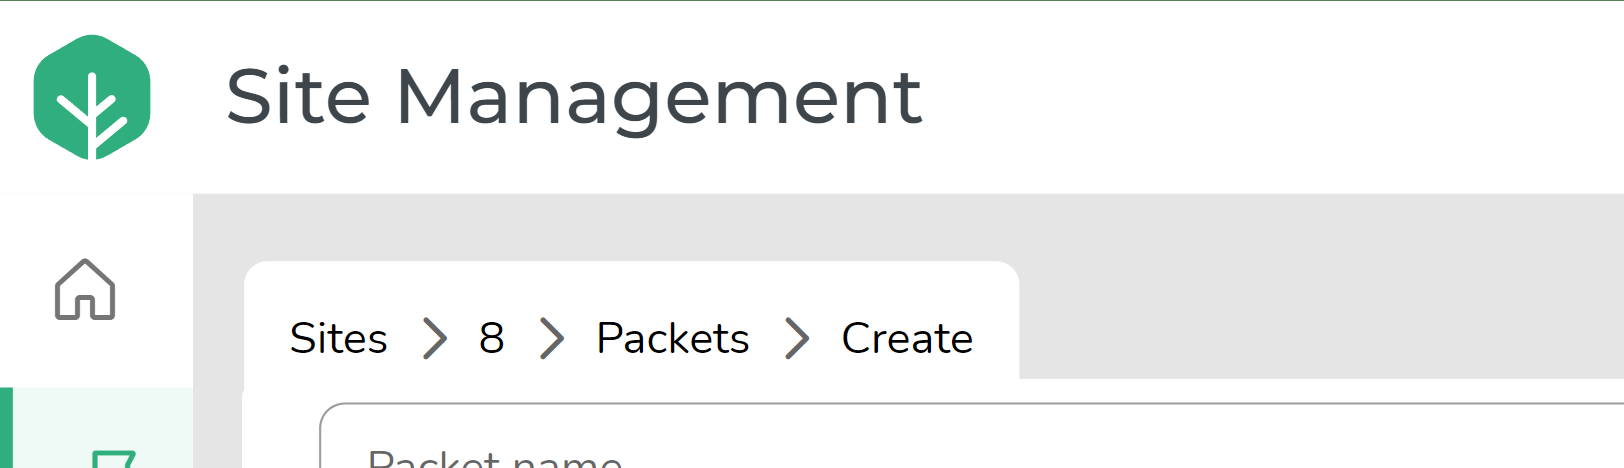
\includegraphics[width=11cm]{app_breadcrumb}
  \caption{Gerenderte breadcrumb-Komponente für den URI \lstinline{/sites/8/packets/_create}}
  \label{fig:app_breadcrumb}
\end{figure}

Die \lstinline{p-breadcrumb}-Komponente wird nicht angezeigt, wenn es weniger als zwei Items gibt.
Dies geschieht einfach in der Vorlage mit einer \lstinline{*ngIf}-Bedingung.

\begin{lstlisting}[
  language=javascript,
  caption={Bedingte Anzeige der Komponente \lstinline{p-breadcrumb} in der Template der customisierten Komponente \lstinline{dryad-breadcrumb}},
  captionpos=b,
]
<p-breadcrumb *ngIf="items.length > 1" [model]="items"></p-breadcrumb>
\end{lstlisting}
